\section{Results}
    \label{sec:results}
    \begin{figure*}
        \centering
        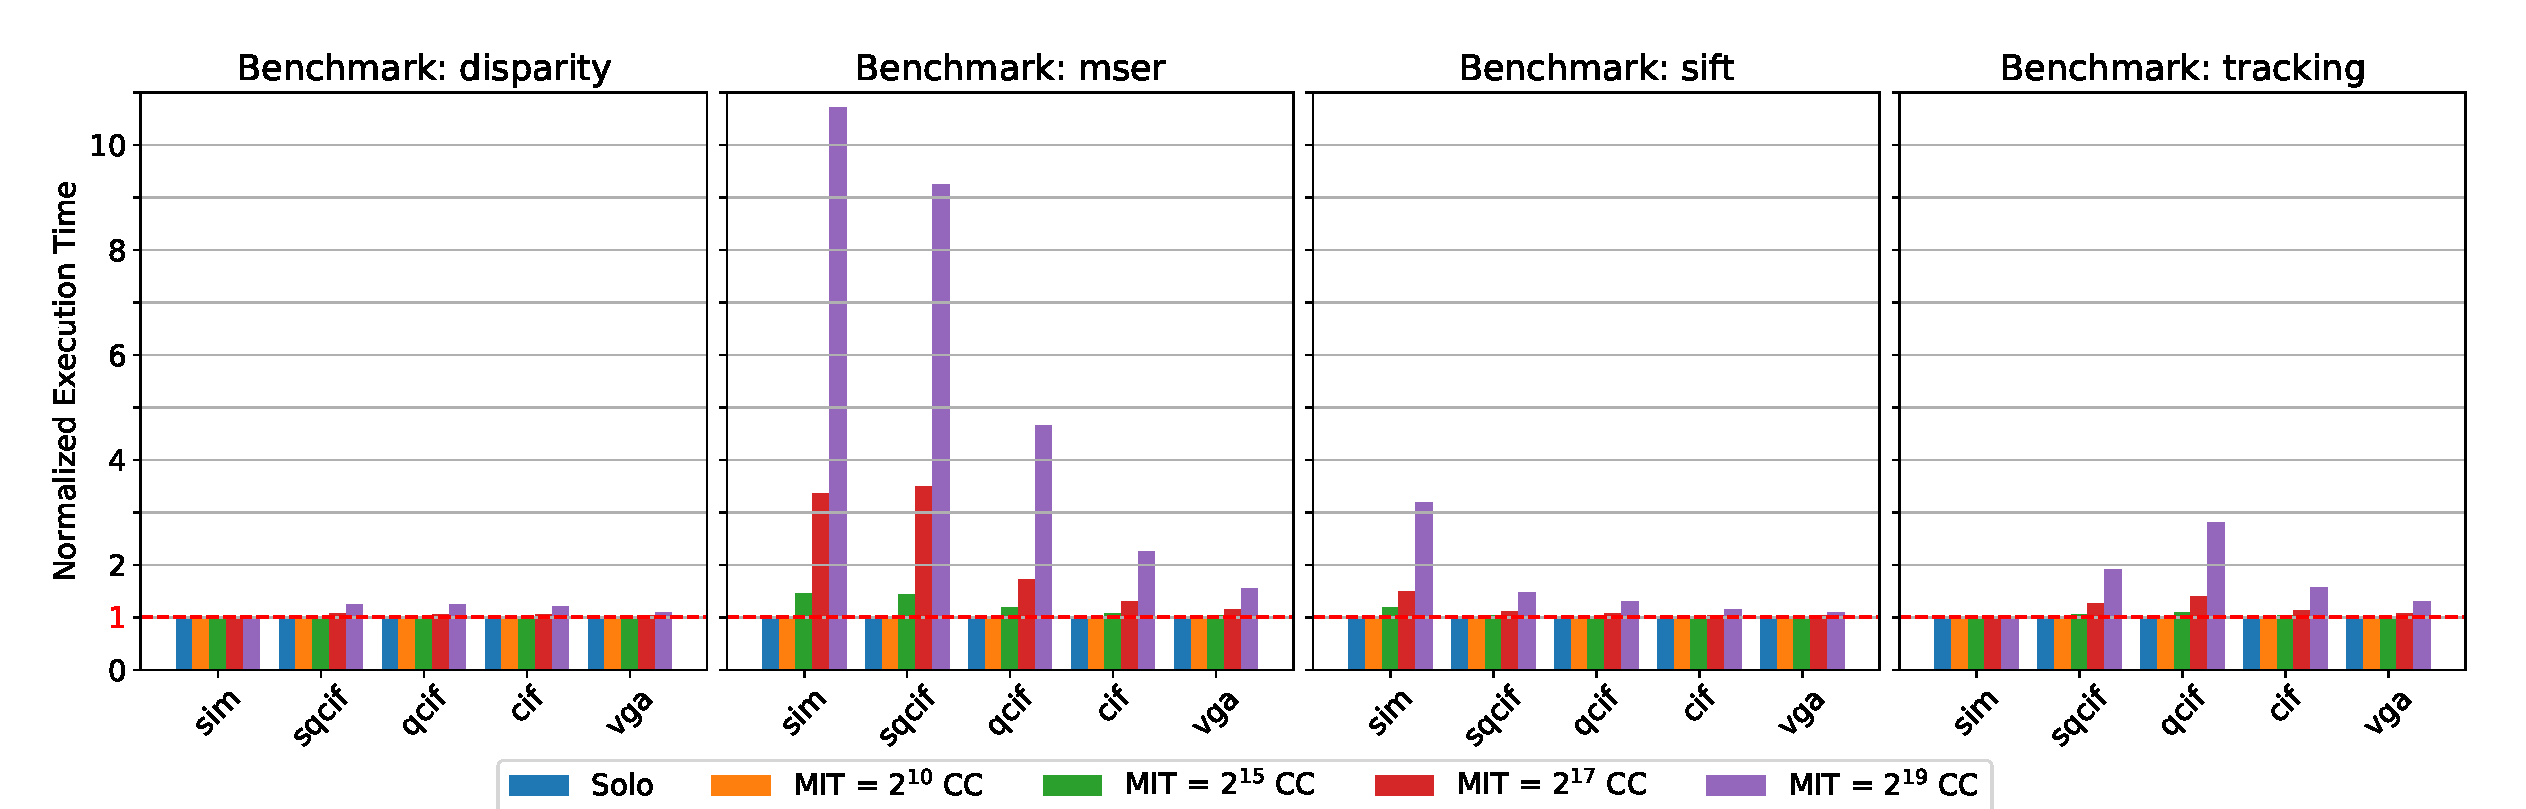
\includegraphics[scale=0.425]{images/cpu-brainfreeze-interference.pdf}
        \caption{Normailized execution time (w.r.t. Solo) for different combinations of benchmark (inset), input sizes (x axis) and MITs for the AXI-Resistor IP (bar color).}
        \label{fig:cpu-brainfreeze-interference-results}
    \end{figure*}

%    \begin{table}
%        \centering
%        \caption{}
%        \label{tab:sd-vbs-input-sizes}
%        \begin{tabular}{|l||c|c|c|c|c|}
%            \hline
%            Input size name  & \emph{sim} & \emph{sqcif} & \emph{qcif} & \emph{cif} & \emph{vga} \\
%            \hline
%            Size in Kilobytes &  $11.7$ &    $36.9$ &   $81.4$ & $304.2$ & $846.8$ \\
%            \hline
%        \end{tabular}
%    \end{table}

    Using the scenario and setup presented in section \ref{sec:evaluation_setup}, we aim at observing the interference caused bu the lightweight read attcker on the victim inmate. To this end, we ran few applicative benchmarks issued from the San-Diego Vision Benchmark Suite \cite{SD-VBS} for all the available input sizes. The benchmarks were also run ffor different configuration of the AXI-Resistor. The latter was configured with MITs of $2^{10}$, $2^{15}$, $2^{17}$ and $2^{19}$. As a baseline, the benchmarks have also been run alone (i.e. without an attacker). This baseline is referred to as "Solo" in Figure \ref{fig:cpu-brainfreeze-interference-results}.

    Figure \ref{fig:cpu-brainfreeze-interference-results} offers a relevant subset\footnote{The complete set of results is available at: URL ommited for review} of results obtained from the experiment. All the results for a given benchmark (localization, mser, sift and tracking) and its size input have been normalized with respect to the equivalent combination running alone (i.e. Solo, the leftmost blue bar in each bar cluster).

    As display in Figure \ref{fig:cpu-brainfreeze-interference-results}, the victim inmate, while running the localization benchmark, suffers from little to no interference from the attacker. The only noticeable increase in execution time is for a \emph{vga} input size and a MIT of $2^{19}$, where the victim suffers from a $150\%$ increase of computation time.
    On the other hand, when running mser, a well known memory bound benchmark, noticeable increases in execution time are observed, with a factor of 10 observed for the \emph{sim} input size.
    For both sift and tracking spikes in execution time are observed. Eventhough, there is no clear pattern with respect to the input sizes, increase in execution time happen for MITs of $2^{17}$ and $2^{19}$.\\

    Interrestingly, configuring the AXI-Resistor in such a way that it would accept the read trasaction, but never answer systematically, leads to the whole system being suspended undefinitely. This can effectively be considered as a Denial-of-Service attack.
